There is a hidden complete binary tree.$^{\dagger}$ Your walk starts at its root.

Each node may have a left child and a right child; every node except the root is connected to its parent.

You do not know the structure of the tree or the total number of nodes. Determine the total number of nodes by moving through the tree using the allowed queries.

For each test case, the number of nodes $N$ satisfies $1 \le N \le 10^{18}$.

\begin{center}
  \def \htmlPixelsInCm {45}
  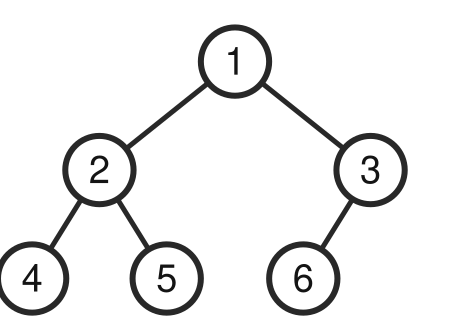
\includegraphics[width=6cm]{cbt.svg} \\[4pt]
  \small{A complete binary tree with $6$ nodes.}
\end{center}

{\small $^{\dagger}$ Formally, a \emph{complete binary tree} is a binary tree in which every level, except possibly the last, is completely filled, and all nodes on the last level are as far to the left as possible. Nodes are numbered in level order from left to right, starting with the root as node $1$.}
